\documentclass[a4paper,12pt,title]{article}
\usepackage{graphicx}
\usepackage{enumerate}
\usepackage{latexsym}
%\usepackage{enumitem}
\usepackage{color}
\usepackage{amsmath}
\usepackage{xcolor}
\usepackage{listings}
\usepackage{caption}
\usepackage{subcaption}
\usepackage[bitstream-charter]{mathdesign}
\usepackage[english]{babel}	
\usepackage[T1]{fontenc}
\DeclareRobustCommand\nobreakspace{\leavevmode\nobreak\ }
\usepackage{titlesec}
\usepackage[top=2cm,bottom=2.5cm,left=2.5cm,right=2.5cm]{geometry}
\usepackage{enumitem}
\usepackage{wrapfig}
\usepackage{ulem}
\usepackage{pdfpages}
%\usepackage{hyperref}
\titleformat{\chapter}{\LARGE\bfseries}{\thechapter}{1em}{}
\usepackage[stable]{footmisc}
\setlist[itemize]{itemsep=0mm}
\DeclareCaptionFont{white}{\color{white}}
\DeclareCaptionFormat{listing}{\colorbox{gray}{\parbox{\textwidth}{#1#2#3}}}
\captionsetup[lstlisting]{format=listing,labelfont=white,textfont=white,skip=-1pt}

\definecolor{lightgray}{rgb}{.9,.9,.9}
\definecolor{darkgray}{rgb}{.4,.4,.4}
\definecolor{purple}{rgb}{0.65, 0.12, 0.82}
\lstdefinelanguage{JavaScript}{
  keywords={typeof, new, true, false, catch, function, return, null, catch, switch, var, if, in, while, do, else, case, break},
  %keywordstyle=\color{blue}\bfseries,
  ndkeywords={class, export, boolean, throw, implements, import, this},
  ndkeywordstyle=\color{darkgray}\bfseries,
  identifierstyle=\color{black},
  sensitive=false,
  comment=[l]{//},
  morecomment=[s]{/*}{*/},
  commentstyle=\color{purple}\ttfamily,
  stringstyle=\color{blue}\ttfamily,
  morestring=[b]',
  morestring=[b]"
}

\lstset{
    xleftmargin=3.5pt,
    xrightmargin =-4.1pt,
    aboveskip= 3pt,
    basicstyle=\small\ttfamily\bfseries,
    frame=lbr,
    language=Javascript,
   extendedchars=true,
   showstringspaces=false,
   showspaces=false,
   tabsize=2,
   breaklines=true,
   showtabs=false,
}
\title{\textsc{\hspace{-15pt} \Large{project report for data mining course}}\\Automatic Review Usefulness Scoring\\ [10pt] \normalsize{Designing a Scoring Model for Yelp's Recruiting Contest\footnote{http://www.kaggle.com/c/yelp-recruiting}}}

\date{\today}

\begin{document}
%\includepdf[pages={1}]{cover.pdf}
\maketitle

\section{Introduction}
Internet nowadays has become a place for both experience showing as well as information hunting. Smart websites bridge the two needs by asking customers to write reviews for the product they have purchased or the service they have used. The reviews have proved to exert considerable influence in people's decision making\cite{mouthonsales}. Yelp\footnote{http://www.yelp.com} is such a website that helps people find local businesses in an area with their past customer's reviews and ratings. It has now covered popular businesses of various categories, including restaurants, bars, shops, beauty \& spas, automotive in United States and countries across Europe. Using large quantity of up-to-date ratings and reviews, Yelp can make recommendation to people in the local.

However, the quality of reviews varies since anyone with Internet access is free to post. Yelp tracks 3 community-powered metrics of review quality: Useful, Funny and Cool. Over time, a good review will accumulate many votes of these categories from the community. However, the freshness of a review is another quality feature, which may allow Yelp to deliver sufficient information to website visitors in time, without having to wait for the communicty votes which have to be accumulated for a long time. The goal of the competition is to estimate the number of Useful votes a review of business will receive to satisfy such need.

By the time this report is written, the proposed model ranked No.20 out of 268 participants\footnote{https://www.kaggle.com/c/yelp-recruiting/leaderboard under name \texttt{ecsark}}.

\section{Data}
The training data set include 11,537 business information (with 8,282 checkin records), 43,873 user profiles and 229,907 reviews in Arizona, United States. 

\begin{lstlisting}[caption=Business]
'business_id': (encrypted business id),
'name': (business name),
'full_address': (localized address),
'city': (city),
'latitude': latitude,
'longitude': longitude,
'stars': (star rating, rounded to half-stars),
'review_count': review count,
'categories': [(localized category names)]
'open': True/False (corresponds to permanently closed, not business hours)
\end{lstlisting}
\begin{lstlisting}[caption=Review]
'user_id': (encrypted user id),
'stars': (star rating),
'text': (review text),
'date': (date, formatted like '2012-03-14'),
'votes': {'useful': (count), 'funny': (count), 'cool': (count)}
\end{lstlisting}
\begin{lstlisting}[caption=User]
'user_id': (encrypted user id),
'name': (first name),
'review_count': (review count),
'average_stars': (floating point average, like 4.31),
'votes': {'useful': (count), 'funny': (count), 'cool': (count)}
\end{lstlisting}
\begin{lstlisting}[caption=Checkin]

'business_id': (encrypted business id),
'checkin_info': {
'0-0': (number of checkins from 00:00 to 01:00 on all Sundays), 
'1-0': (number of checkins from 01:00 to 02:00 on all Sundays), 
... 
'14-4': (number of checkins from 14:00 to 15:00 on all Thursdays), 
... 
'23-6': (number of checkins from 23:00 to 00:00 on all Saturdays)
}
\end{lstlisting}

The test data format is slightly different from that of the training set in that neither \texttt{Review} and \texttt{User} does not contain \texttt{votes} information any more. Also note that a reviewer may keep his/her profile private, which means that no information about the user can be found in the data set.


\section{Review Usefulness Features}
This section describes the features used in the model and explains their relevance.

\subsection{Entity Attributes Perspective}
Entity attributes refer to features not derived by analyzing the text, which involves the star ratings included in the review, the date the reviews was written, business features and user characters.

Reviews were written in a span over 8 years(from 2005/03 to 2013/01), making old reviews obesolete to earn new votes while leaving fresh ones little time to gain community recognition. An asymmetric bell curve can be observed in Figure~\ref{fig:vote2date}. Albeit not directly linked to usefulness, review date has proved to be of considerable importance in calculating the votes received on a fixed date.

\begin{figure}
\centerline{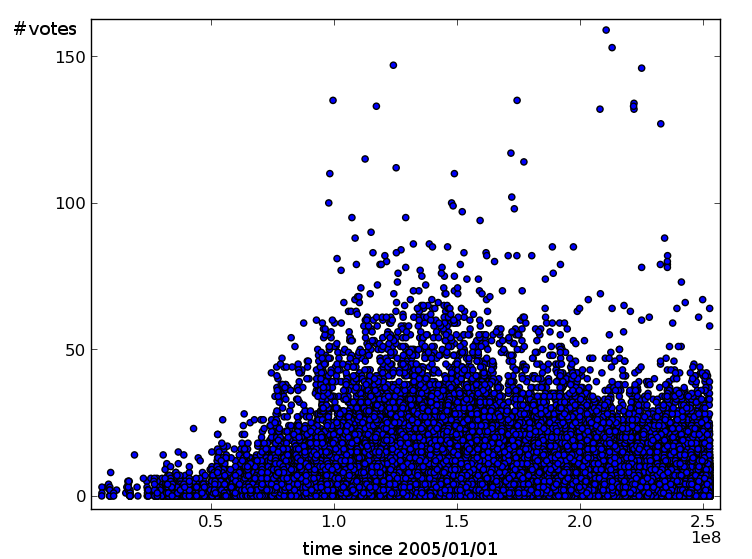
\includegraphics[width=300pt]{graph/vote2date.png}}
\caption{Timeliness of review usefulness votes}
\label{fig:vote2date}
\end{figure}

Review stars are also relevant in review useful assesment. According to the \textit{conformity hypothesis} summarized by Danescu-Niculescu-Mizil et al.\cite{communityreceiveopinion}, review is evaluated as more useful when its star rating is closer to the consensus star rating. However, Yelp's review data gives completely different conclusions. Considering that some businesses enjoy more popularity than others, there exists a vote bias in reviews: popular businesses tend to have their reviews read more often than those of less popular businesses, and leading to more useful votes. Therefore, a score is calculated to assess a review of its usefulness ranking in the scope of reviews written for a specific business. 

$$score = \frac{(votes_{review}+1)\times \#reviews_{bz}}{total votes_{bz}+1}$$

 In Figure~\ref{fig:deviation2score}, one can observe that negative reviews (indicated by their star ratings below average) are more likely to be regarded useful. It might be the fact that negative reviewers are perceived as more intelligent, competent and expert than positive reviewers. And customers tend to remember awful experience and thus giving useful votes to reviews offering similar sentiment .

\begin{figure}
\begin{minipage}[t]{0.5\linewidth}
\centering
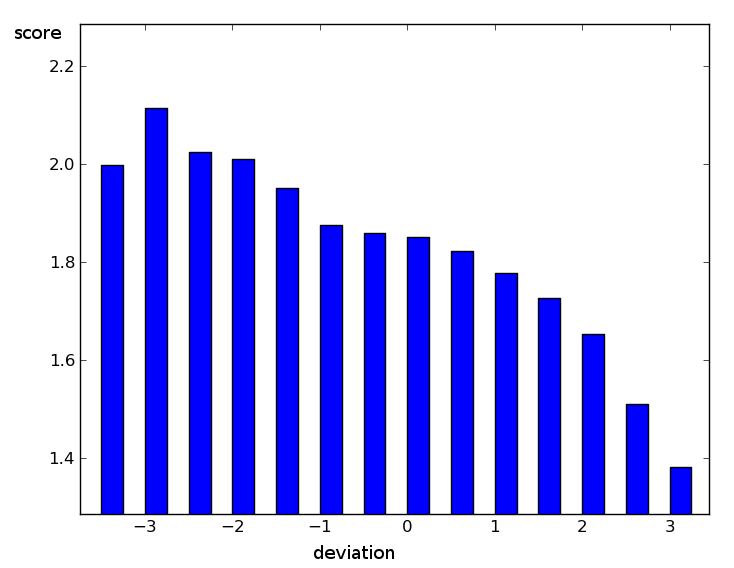
\includegraphics[width=230pt]{graph/starsdeviation.png}
\subcaption{signed deviation}
\label{fig:signed}
\end{minipage}
\begin{minipage}[t]{0.5\linewidth}
\centering
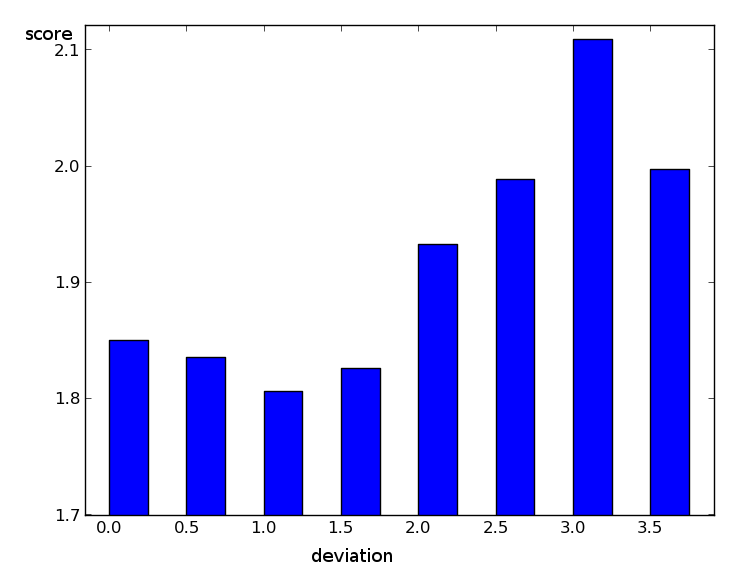
\includegraphics[width=230pt]{graph/abs_starsdeviation.png}
\subcaption{absolute deviation}
\label{fig:unsigned}
\end{minipage}
\caption{Usefulness Score vs. Star Rating Deviation}
\label{fig:deviation2score}
\end{figure}

 Among all entity attribute features, the number of reviews that a user has written is the most interesting. Figure~\ref{fig:rvcount2vote} shows the distribution of reviews against user attributes. In Figure~\ref{fig:macro} one can observe that experienced authors (who has written many reviews) have higher expected (average) quality of reviews. Figure~\ref{fig:micro} shows that when an author has less than 50 reviews, the chance of the review obtaining one useful vote is about a half, which applies to the majority reviews.

\begin{figure}
\begin{minipage}[t]{0.5\linewidth}
\centering
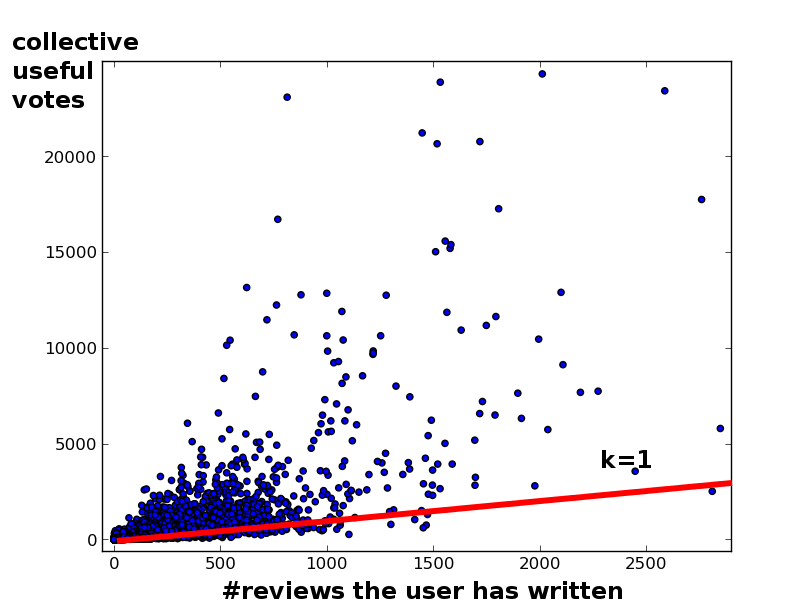
\includegraphics[width=250pt]{graph/reviewcount2votes.png}
\subcaption{macro view}
\label{fig:macro}
\end{minipage}
\begin{minipage}[t]{0.5\linewidth}
\centering
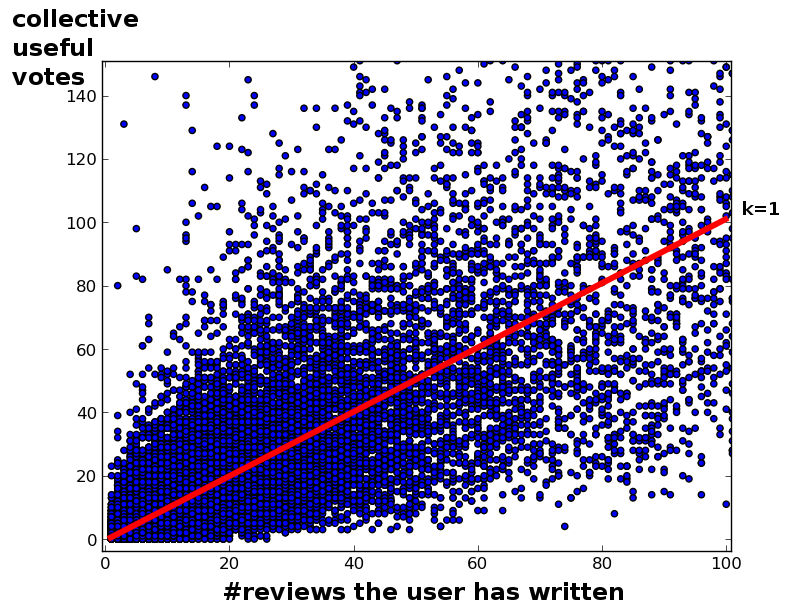
\includegraphics[width=250pt]{graph/reviewcount2votes_mic.png}
\subcaption{micro view}
\label{fig:micro}
\end{minipage}
\caption{Review Count vs. Collective Useful Votes}
\label{fig:rvcount2vote}
\end{figure}

From the business perspective, city and business type (category) mark the regional characteristics, while the total check-in and reviews count are good indicators of the business popularity. The total and average useful votes of reviews are also calculated for each business. As will be shown later, they play important roles in predicting the true useful votes.

\subsection{Textual Perspective}
The most instinct feature in textual analysis is text length. Figure~\ref{fig:length} shows a virtual linear relationship between the reviews' text length and their usefulness score before the words count exceeds 400. It is noted that the info-length, i.e. the length of text removed of stopwords can be a better feature than the full text length.

\begin{figure}
\centerline{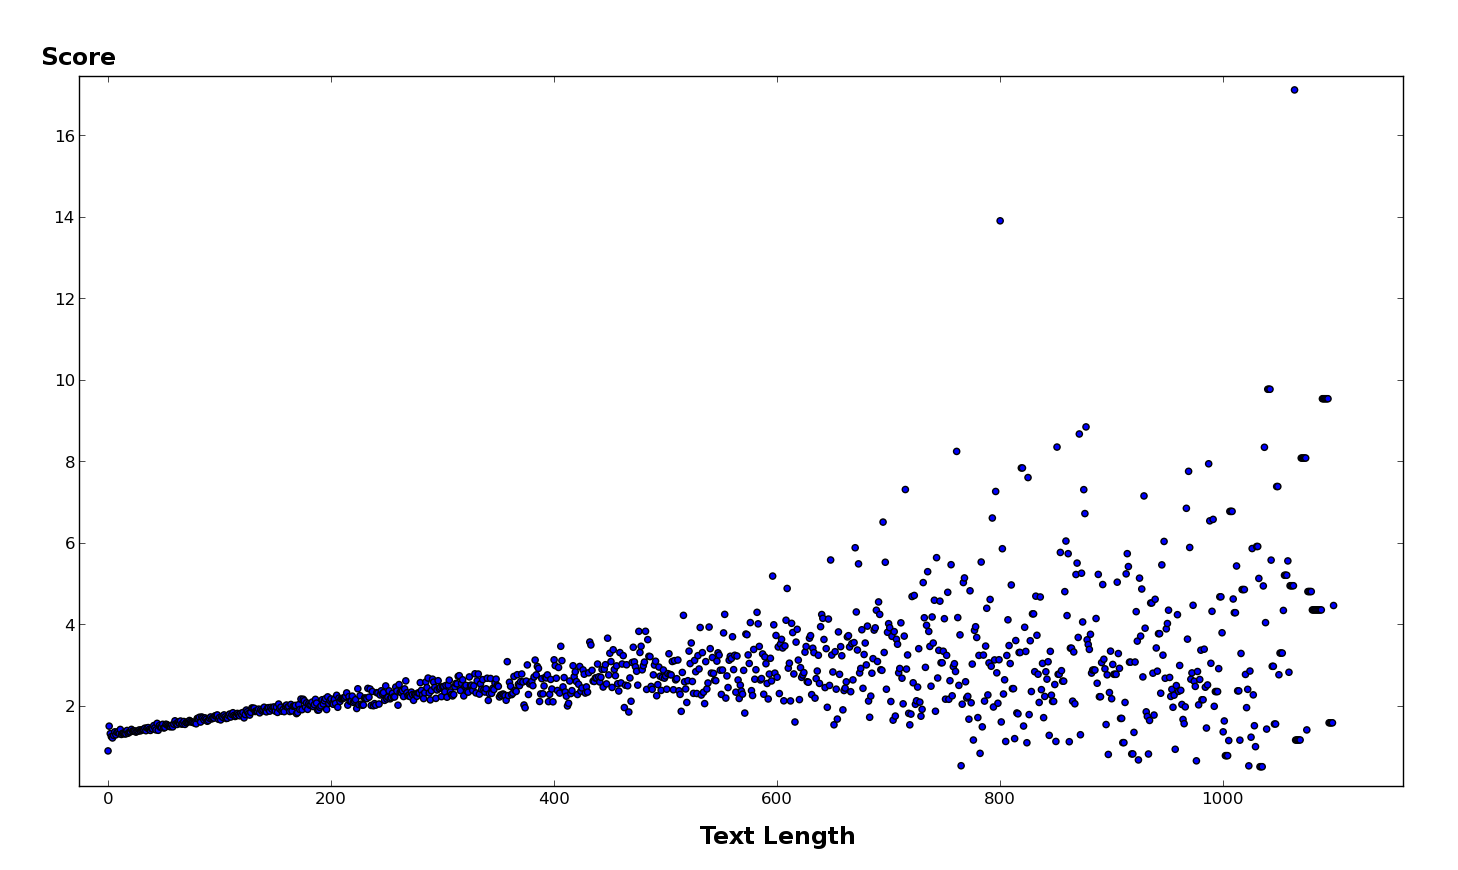
\includegraphics[width=500pt]{graph/length_score.png}}
\caption{Text Length's Contribution to Usefulness}
\label{fig:length}
\end{figure}

Deeper analysis of the review is related to opinion and sentiment mining as well as text classification.

Opinion and sentiment mining focuses on two properties of the text: subjectivity - whether the style of the sentence is subjective or objective; and polarity - whetherthe author is expressing positive or negative opinion. Hu and Liu had a comprehensive study\cite{summarizeopinion} on this task. As proposed in their paper, Part-of-Speech Tagging \textit(POS) can help find opinion features and association mining technique\cite{apriori} can be used to find feature phrases.

Using POS tagger provided in the NLTK package, the model counts the number of words of different categories. For example, the number of nouns (NN), together with proper nouns (NNP \& NNPS, such as Motown, Shannon) can help show the degree of informativeness, whilst pronouns (PRP \& PRP\$, such as me, his, she) are used to represent degree of subjectivity. Adjectives and adverbs are ideal polarity expressions. The true polarity is not being distinguished in this project since the star ratings is included in the reviews. The comparative and superlative form of adjectives and adverbs are also included in the feature set to indicate the degree of subjectivity. 

Bag-of-words is widely used in text classification systems. Soo-Min Kim et al.\cite{empirical} (and many others) suggested that unigram outperforms others with regard to usefulness rating. Its dimension reduced vector was used to train a support-vector-regressor \textit{(SVR)} but has not expected ideal results.

\section{Regression Model \& Experiment}
Two approaches was used to perform regression on useful votes with high dimension feature.

The Support-Vector-Regression \textit{(SVR)} works in similar ways as Support-Vector-Machine \textit{(SVM)} except that SVR tries to find a hyperplane to predict the target data distribution. The target (useful votes) is transformed to its logarithm: $log(useful\_votes+1)$. Using \texttt{sklearn}'s SVR module with radial basis function kernel and a hard iteration limit of 10000, the 3-fold cross validation reports an average 0.6895 Meaned Squared Error \textit{(mse)}.

Random forest is an ensemble method that combines the predictions of several decision trees to improve generalizability and robustness over a single model. Each tree in the ensemble is built from a sample drawn with replacement from the training set. Also, when splitting a node during the construciton of a tree, the split is picked for the best among a random subset of features instead of among all the features. Compared with SVR, decision trees are easy to build and therefore random forest, even run with over a hundred estimators, is much faster to train. 

\texttt{sklearn}'s \texttt{RandomForestRegressor} implementation combines the result of trees by averaging their probabilistic prediction. With 100 trees and Meaned Squared Error \textit{(mse)} as the split criterion, the model produces an average mse of 0.4518 in 3-fold cross validation. 

\begin{center}
\begin{tabular}{rlc}
\textbf{Feature ID} & \textbf{Feature Name} & \textbf{Importance}\\
\hline
\hline
\bfseries{1} & \bfseries{rev\_infolen} & \bfseries{7.28130348e-03}\\
\bfseries{2} & \bfseries{rev\_textlen} & \bfseries{3.09150384e-03}\\
3 & rev\_inforatio & 5.59585832e-05\\
4 & rev\_stars & 2.80702933e-04\\
\bfseries{5} & \bfseries{rev\_date} & \bfseries{5.81661004e-03}\\
6 & txt\_nouns & 4.93268201e-05\\
7 & txt\_proper\_nouns & 5.69934145e-05\\
8 & txt\_pronouns & 4.76200385e-05\\
9 & txt\_adverbs & 5.82525793e-05\\
10 & txt\_adjectives & 5.57349800e-05\\
11 & txt\_comparative & 2.46351008e-05\\
12 & txt\_superlative & 2.27906836e-05\\
13 & txt\_determiner & 4.74415258e-05\\
14 & txt\_conjunction & 4.62229851e-05\\
15 & txt\_pre-determiner & 7.05338308e-06\\
16 & txt\_verbs & 4.31074789e-05\\
17 & txt\_verbs\_present & 4.46257521e-05\\
18 & txt\_verbs\_past & 4.45631220e-05\\
19 & txt\_wh & 2.67373771e-05\\
20 & txt\_modal & 3.43049385e-05\\
21 & bz\_rvcnt & 7.36381727e-05\\
22 & bz\_stars & 3.01277864e-05\\
23 & bz\_city & 2.65306335e-05\\
24 & bz\_category & 3.81247290e-05\\
25 & bz\_checkins & 5.60371119e-05\\
26 & bz\_usefulcnt & 4.74327268e-04\\
27 & bz\_votescnt & 1.96181781e-04\\
28 & bz\_uvotesratio & 2.31708525e-04\\
29 & usr\_rvcnt & 1.40651450e-04\\
30 & usr\_avgstar & 8.83297435e-05\\
\bfseries{31} & \bfseries{usr\_usefulcnt} & \bfseries{9.75049518e-03}\\
32 & usr\_votescnt & 1.91604651e-04\\
\bfseries{33} & \bfseries{usr\_avguvotes} & \bfseries{1.30694998e-01}\\
\bfseries{34} & \bfseries{usr\_avgvotes} & \bfseries{8.40082522e-01}\\
35 & rev\_stardevbz & 9.90989382e-05\\
36 & rev\_stardevusr & 6.36680205e-04\\
37 & usr\_stardevbz & 5.34551884e-05
\end{tabular}
\end{center}

It can be observed that users' past useful votes and meta-data of reviews carry the most importance in decision trees. However, if business is not found in the training set, feature 26,27,28 would not be available in prediction. If user's information is found in test set, feature \textbf{31},32,\textbf{33},\textbf{34},37 would not be available. If user's information is not found either in test nor training set, feature \textbf{31},32,\textbf{33},\textbf{34},36,37 would not be available.  Therefore, 6 independent random forest regressors were trained to cope with their respective cases. 

\begin{center}
\begin{tabular}{cccc}
\textbf{Forest ID} & \textbf{Bz in training set?} & \textbf{Usr in test set?} & \textbf{Usr in training set?}\\
\hline
\hline
000 & No & No & No\\
010 & No & Yes & No\\
011 & No & No & Yes\\
100 & Yes & No & No\\
110 & Yes & Yes & No\\
111 & Yes & No & Yes\\
\end{tabular}
\end{center}

Finally, the test data which combines the 6 situations above, scored 0.46446 mse.

\section{Future Work}
Because of the limited time and computing ability of my laptop, I have only used two regression models. Feature set contains only a few helpful indicators with regard to usefulness rating. In the future, more textual analysis is desired, such as entity recognition, uniqueness assessment, spam detection. Furthermore, regression models can be build at a finer granularity, such as at category level.

\begin{thebibliography}{9}
\bibitem{mouthonsales}\textsc{Chevalier, J. A., and Mayzlin, D.} The effect of word of mouth on sales: Online book reviews. \textit{Journal of Marketing Research} 43, 3 (Aug. 2006), 345–354.
\bibitem{communityreceiveopinion}\textsc{Cristian Danescu-Niculescu-Mizil, Gueorgi Kossinets, Jon Kleinberg, and Lillian Lee} How Opinions are Received by Online Communities: A Case Study on Amazon.com Helpfulness Votes. \textit{WWW}, April 20–24, 2009
\bibitem{summarizeopinion}\textsc{Minqing Hu, Bing Liu} Mining and Summarizing Customer Reviews. \textit{KDD'04}, Aug 22–25, 2004
\bibitem{apriori}\textsc{Rakesh Agrawal, Ramakrishnan Srikant} Fast Algorithms for Mining Association Rules. \textit{Proceedings of the 20th VLDB Conference}, Santiago, Chile, 1994
\bibitem{empirical}\textsc{Soo-Min Kim, Patrick Pantel, Tim Chklovski, Marco Pennacchiotti} Automatically Assessing Review Helpfulness. \textit{Proceedings of the 2006 Conference on Empirical Methods in Natural Language Processing}, Sydney, July 2006, pages 423–430
\bibitem{satisfactory} \textsc{Yu Hong, Jun Lu, Jianmin Yao, Qiaoming Zhu,Guodong Zhou} What Reviews are Satisfactory: Novel Features for Automatic Helpfulness Voting. \textit{SIGIR’12}, August 12-16, 2012, Portland, Oregon, USA
\bibitem{shortessay} \textsc{Luis Tandalla} Scoring Short Answer Essays. \textit{The Hewlett Foundation: Short Answer Scoring Contest}, https://www.kaggle.com/c/asap-sas/details/preliminary-winners
\end{thebibliography}
\end{document}
